\subsection{Orbit dynamics}
    \dots\textit{work in progress}\dots

    \begin{equation}
        \begin{bmatrix}  \delta\dot{u} \\ \delta\dot{v} \\ \delta\dot{w} \\ \delta\dot{x} \\ \delta\dot{y} \\ \delta\dot{z} \end{bmatrix}
        =
        \begin{bmatrix}
        0 & 0 & 0 & -n^2 & 0 & 0 \\
        0 & 0 & 0 & 0 & -n&2 & 0 \\
        -n & 0 & 0 & 0 & 0 & 2n^2 \\
        1 & 0 & 0 & 0 & 0 & 0 \\
        0 & 1 & 0 & 0 & 0 & 0 \\
        0 & 0 & 1 & -1 & 0 & 0
        \end{bmatrix}
        \begin{bmatrix}  \delta u \\ \delta v \\ \delta w \\ \delta x \\ \delta y \\ \delta z \end{bmatrix}
        +
        \begin{bmatrix}
        T_x/m \\
        T_y/m \\
        T_z/m \\
        0 \\
        0 \\
        0
        \end{bmatrix}
    \end{equation}\label{eqn:sstranslation}
    For small attitude changes of non-spinning spacecraft with respect to inertial frame, equations describing rotational motion can be linearized. The acquired system is then:
    \begin{equation}
        \begin{bmatrix}
        \dot{p} \\
        \dot{q} \\
        \dot{r} \\
        \dot{\Phi} \\
        \dot{\Theta} \\
        \dot{\Psi}
        \end{bmatrix}
        =
        \begin{bmatrix}
            0 & 0 & 0 & 0 & 0 & 0 \\
            0 & 0 & 0 & 0 & 0 & 0 \\
            0 & 0 & 0 & 0 & 0 & 0 \\
            1 & 0 & 0 & 0 & 0 & n \\
            0 & 1 & 0 & 0 & 0 & 0 \\
            0 & 0 & 1 & -n & 0 & 0 \\ 
        \end{bmatrix}
        \begin{bmatrix}
            p \\
            q \\
            r \\
            \Phi \\
            \Theta \\
            \Psi
        \end{bmatrix}
        +
        \begin{bmatrix}
            Q_x/I_x \\
            Q_y/I_x \\
            Q_z/I_z \\
            0 \\
            n \\
            0
            \end{bmatrix}
    \end{equation}\label{eqn:ssrotation}
    Where $n=\sqrt{g/R_E}$ is satellite's orbital angular velocity.

\subsection{Spacecraft Mechanics}
    % https://www.mathworks.com/discovery/linearization.html
    Spacecraft mechanics are governed by the laws describing the motions of a body under the influence of external and internal forces and torques. Forces acting on a spacecraft influence its translational motion, which in the simplest form can be described as a set of differential equations in a form of $\dot{x} = Ax + Bu$. In this case, $x$ is a state vector built from satellites position vector in three-dimensional Cartesian coordinates and first order derivatives of said vector. For simplified point-on-orbit satellite 

    One of the goals of this thesis is to create means to design a satellite control system for people without much experience in that field. One of the ways to accomplish that is to eliminate the need to derive complex mathematical models of the systems involved. Nevertheless, there exists a need for such models, for example for LQR control algorithm described in Section \ref{sec:lqr}. One could try to further develop Equations \ref{eqn:sstranslation} and \ref{eqn:sstranslation} into state-space representation of whole spacecraft system including all actuators and sensors, parametrize it and programmatically modify it, for each configuration, to include only set-up parts. Alternative solution it to use MATLAB Control System Toolbox and its functions to automatically linearize Simulink models. The main advantage of this solution is that it also encompasses all changes from the users to the \ac{scars} Modular Simulation. The process is described in \autoref{app:linearization}.

    A mathematical model can be used in analytical solutions, but in 
    
    A Spacecraft Model block in \ac{scars} is built around Simulink Aerospace Blockset 6DOF ECEF (Quaternion) block.

    \dots\textit{finish the explanation}\dots

\subsection{Reference Frames}
    % \dots\textit{introduction}\dots
    To find the states of the chosen object, one has to first describe the coordinate system and the reference points used for this definition. Most useful ones from the perspective of the spacecraft \ac{aocs} design are described below and their relationship is showed on \autoref{fig:frames}.

    \begin{figure}[H]
        \centering
        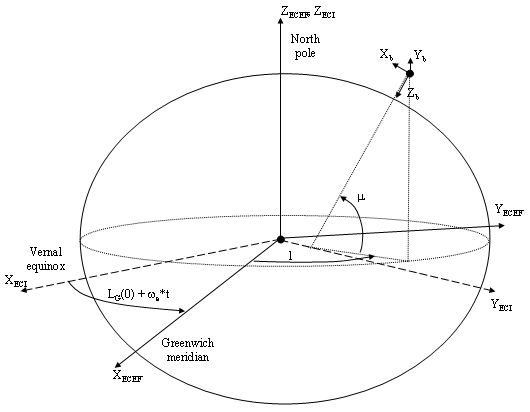
\includegraphics[width=1\textwidth]{2-toolbox/frames.png}
        \caption{Satellite Reference Frames\cite{6ecef-frames}}
        \label{fig:frames}
    \end{figure}

    \subsubsection{Satellite Body Frame}
        \dots\textit{description of implementation}\dots
        Satellite Body Frame has its origin at the center of mass of the spacecraft, with axes directions chosen to fit the design of the spacecraft. For example, for observation missions, most often one of the axes corresponds to the axis of satellite's optical instrument.

    \subsubsection{\ac*{ned}}
        \ac{ned} is a local tangent plane coordinate frame. It is fixed to the body of the satellite, with $Z_{NED}$ axis pointing towards the center of the Earth, $X_{NED}$ axis oriented in the direction of north and $Y_{NED}$ towards east. The most popular application of \ac{ned} frame is for aircraft and spacecraft, when most objects of interest are below the vehicle, therefore it is convenient to be able to reference the position of the target with positive value.

    \subsubsection{\ac*{eci}}
        The \ac{eci} frame has its origin located in Earth's center of gravity. It has $X$ axis parallel to and directed as vernal equinox direction, its $Z$ axis is constructed from the vector starting in origin and going through Earth's celestial North pole and $Y$ axis is a vector cross product of the other two. Specific \ac{eci} frame used in this thesis is J2000 frame, defined with with the Earth's Mean Equator and Equinox at 12:00 Terrestrial Time on 1 January 2000 \cite{schutz2004statistical}. Position and velocity vectors in this frame will be further noted as $\textbf{r}_\textbf{ECI}$ and $\textbf{v}_\textbf{ECI}$ respectively.

    \subsubsection{\ac*{ecef}}
        % \ac{ecef}, also known as \ac{ecr}, frame of reference can be derived from \ac{eci} frame by including information about Earth's rotation.
        The \ac{ecef}, also known as \ac{ecr}, is a frame of reference can with origin in Earth's center of mass and it's axes are parallel with international reference pole ($Z_{ECEF}$ axis) and international reference meridian ($X_{ECEF}$ axis), with $Y_{ECEF}$ axis being vector cross product of other two. The \ac{ecef} frame includes information about rotation of the Earth, hence a point which would be fixed in the \ac{eci} frame would be progressing with time in the \ac{ecef} frame. Vectors in this frame will be further noted as $\textbf{r}_{\textbf{ECEF}}$ and $\textbf{v}_{\textbf{ECEF}} $.
        %todo: find citation


\subsection{Coordinates Transformations}
    Since for different purposes various reference frames and coordinate systems have to be used, it is necessary to have the means to transform vectors between them. As for reference frames the solution is to find a \ac{dcm}, that is a 3-by-3 matrix which can be used to transform three-dimensional vector $\textbf{x}$ into another vector $\textbf{y}$ with the following equation:
    \begin{equation}
        \textbf{y} = DCM\textbf{x}
    \end{equation}
    As coordinate transformations are more complex, each one is described in its respective subsection. All transformations are implemented within \ac{scars} Toolbox as the algorithms presented and masked for ease of use.
    % Note (vel eci to ecef): https://github.com/JuliaSpace/SatelliteToolbox.jl/issues/5
    
    \subsubsection{\ac{eci} position and velocity vector to Keplerian elements}
        As mentioned, Earth orbiting satellite's position can be described by it's position vector $\textbf{r}$ in Cartesian coordinate system, with center corresponding to Earth's geometric center. That vector in connection with spacecraft's velocity vector $\textbf{v}$ in same coordinate system can be transformed into Keplerian elements by using following equations:
        \begin{align}
            a &= \frac{\mu}{2\left(\frac{\mu}{r}-\frac{v^2}{2}\right)} \\
            i &= \cos^{-1}(\frac{h_Z}{|\textbf{h}|} \\
            e &= \sqrt(\frac{1-h^2}{\mu a}) \\
            \psi &= \cos^{-1}\left(\frac{a-|\textbf{r}|}{ae}\right), \; where \; \sin(\psi) = \frac{\textbf{r}\cdot\textbf{v}}{e\sqrt{\mu a}} \\
            \theta &= \sin^{-1}\left[\frac{\sin(\psi \sqrt{1-e^2})}{1-e\cos(\psi)}\right] \\
            M & = \psi - e\sin(\psi)
        \end{align}
        And $\Omega$ and $\omega$ can be found from following relations:
        \begin{align}
            \sin(\Omega) = \frac{h_X}{\sqrt{h^2_X+h^2_Y}}\; & and\; \cos(\Omega) = \frac{h_Y}{\sqrt{h^2_X+h^2_Y}} \\
            \sin(\omega+\theta) = \frac{r_Z}{r\sin(i)}\; & and\; \cos(\omega+\theta) = \frac{r_Z\cos(\Omega)+r_Y\sin(\Omega)}{r}
        \end{align}
        Where terms $h_X$, $h_Y$ and $h_Z$ are components of $\textbf{h}=\textbf{r}\times \textbf{v}$ vector and $r_X$, $r_Y$ and $r_Z$ are components of position vector.
    
    \subsubsection{Keplerian elements to \ac{eci} position and velocity vector}
        To quickly obtain position vector from Keplerian elements one may define a coordinate system with $x$, $y$ axes on orbit's plane with $z=0$. Then the following equations describe the coordinates:
        \begin{align}
            x & = a\cos(\psi) -ae \\
            y &= a\sin(\psi)\sqrt{1-e^2}
        \end{align}
        Then the position in Earth's inertial Cartesian coordinate system can be found with following system of equations:
        \begin{align}
            \textbf{r} = \begin{bmatrix} r_X\\ r_Y\\ r_Z \end{bmatrix} = [A_Z(\Omega)]^{-1} [A_X(i)]^{-1} [A_Z(\omega)]^{-1} \begin{bmatrix} x\\ y\\ 0 \end{bmatrix}
        \end{align}
        Where $[A_d(\alpha)]$ stands for transformation matrix about axis $d$ by an $\alpha$ angle.
        % You have interesting stuff in PW-Sat2 ADCS CDR :)
        %todo: Write about velocity here
        %SIDI 25 (43 in foxit)        
        %  Citation for orbital elements: \cite{vallado2001fundamentals}

    \subsubsection{\ac{eci} to \ac{ecef}}
        To transform vectors calculated in inertial frame to Earth-Fixed reference frame one has to multiply the \ac{eci} vector by following rotation matrix:
        \begin{equation}
            DCM^{ECI}_{ECEF} = \begin{bmatrix} \cos\theta_{GMST} & \sin\theta_{GMST} & 0\\
            -\sin\theta_{GMST} & \cos\theta_{GMST} & 0 \\
            0 & 0 & 1 \end{bmatrix}
        \end{equation}
        Where $\theta_{GMST}$ is Earth's rotation angle; to be calculated with:
        \begin{multline}
        \theta_{GMST}= \frac{1}{240} \cdot \mod[24110.54841 + 8640185.812866 \cdot Y + 0.093104 \cdot Y^2 \\
            - 6.2*10^{-6} \cdot Y^3 + 1.002737909350795\left(3600hh+60mm+ss\right), 8640]
        \end{multline}
        Where $Y$ is the number or Julian centuries elapsed from the J2000 epoch and $\mod{a,b}$ is the modulo operator.

    \subsubsection{\ac{ecef} to \ac{ned}}
       Implementation of this transformation assumes that the origin of \ac{ecef} frame is at the center of the planet, the $X_{ECEF}$ axis intersects the Greenwich meridian and the equator, the $Z_{ECEF}$ axis is the mean spin axis of the planet, positive to the north, and the $Y_{ECEF}$ completes the right-hand system \cite{aboutareospace}. The following equation shows the \ac{dcm} for that transformation:
       \begin{equation}
           DCM^{ECEF}_{NED} = \begin{bmatrix} -\sin\phi\cos\lambda & -\sin\phi\sin\lambda & \cos\phi\\
               -\sin\lambda & \cos\lambda & 0 \\
               -\cos\phi\cos\lambda & -\cos\phi\sin\lambda -\sin\phi \end{bmatrix}
       \end{equation}

    \subsubsection{\ac{ecef} to \ac{lla}}
        One can calculate geodetic longitude $\lambda$ with ease, by following the simple relation:
        \begin{equation}
            \\lambda = \arctan(\frac{Y_{ECEF}}{X_{ECEF}})
        \end{equation}
        But to find the geodetic latitude $\phi$ Bowring's iterative method has to be employed \cite{gerdan1999transforming}. The calculations are performed inside the \ac{scars} Satellite Model and can be read from the workspace after the simulation is run at least once.

        \dots\textit{the explanation}\dots

% The body is assumed to be rigid?
% Non perturbed orbit?


\subsection{Environment}
    % Environment block is responsible for outputting few parameters, which are then used by the Satellite subsystem
    Environment module is responsible for producing environmental parameters such as gravity, magnetic field, atmosphere density, etc., at the position of the simulated spacecraft. The reasoning behind choosing these specific sources are in the description of each sub-module. The main premise was that the source has to be relevant for the choice of actuators.
    
    \subsubsection{Earths's Gravity Model}
        Main centripetal force acting on a spacecraft on any orbit is gravity - it is defined by the equation derived from the law formalized by Isaac Newton:
        \begin{equation}
            \ddot{\textbf{r}} = -\frac{G(m_1+m_2)\textbf{r}}{\left\Vert \textbf{r} \right\Vert^2}
        \end{equation}

        Where $r$ is the position vector, $m_1$ and $m_2$ are the masses of two-body system and $G$ is the universal gravitational constant. Simplified with:
        \begin{equation}
            m_1 = M_{Earth} \gg m_2 = m_{spacecraft}
        \end{equation}
        One can derive the corresponding potential function:
        \begin{equation}
            u = -\frac{GM_{Earth}}{\textbf{r}}\label{eq:pot}
        \end{equation}
        For a spacecraft on Earth's orbit, this model is a very far-stretched approximation, as it leaves out the influence of Earth's non-ideal shape, changes in density gradient in Earth's interior and perturbations caused by gravitational fields of other bodies. While the influence of other celestial objects is omitted in the \ac{scars} toolbox due to it being mostly designed for lower orbits, one can easily account for Earth's non-spherical mass distribution using function constructed with the use of Lagendre polynomials to calculate the correction $\epsilon$ to potential function \eqref{eq:pot}:

        \begin{equation}
            \epsilon(r, \theta, \varphi) = \sum_{n=2}^{\infty}  \frac{J_n P^0_n(\sin\theta) }{r^{n+1}} + \sum_{n=2}^{\infty} \sum_{m=1}^n \frac{ P^m_n(\sin\theta) (C_n^m \cos m\varphi + S_n^m \sin m\varphi)}{r^{n+1}}\label{eq:geopot}
        \end{equation}

        Where the correction is a function of spacecraft's position in spherical coordinate system - $r$, $\theta$, $\varphi$ are in order altitude, latitude and longitude. The coefficients $J_n$, $C_n^m$ and $S_n^m$ are computed to possibly provide best approximation between observed and calculated orbit. Lagendre polynomials of form 
        \begin{equation}
            \frac{P^0_n(\sin\theta) }{r^{n+1}}    
        \end{equation}
        are called the zonal terms and Lagendre functions 
        \begin{equation}
        \begin{aligned}
            \frac{ P^m_n(\sin\theta) \cos m\varphi}{r^{n+1}}\\
            \frac{ P^m_n(\sin\theta) \sin m\varphi}{r^{n+1}}
        \end{aligned}
        \end{equation}
        correspond to tesseral terms. The denominating term is the so-called "J\textsubscript{2} term":

        \begin{equation}
            \frac{J_2\ P^0_2(\sin\theta)}{r^3} = J_2 \frac{1}{r^3} \frac{1}{2} (3\sin^2\theta -1) = J_2 \frac{1}{r^5} \frac{1}{2} (3 r^2sin^2\theta -r^2)
        \end{equation}

        While equations \eqref{eq:pot} and \eqref{eq:geopot} can added together to faithfully model the influence of Earth's gravity field on the spacecraft, it was decided to use a model from Simulink Aerospace Blockset - the Spherical Harmonic Gravity Model, with EGM2008 planetary model, as it is much more detailed and provides better accuracy.

        % Potentialy relevant: https://www.mathworks.com/matlabcentral/answers/349791-simulink-spacecraft-motion-integration-using-spherical-harmonic-gravity-model-problem

    \subsubsection{Partial Atmosphere}\label{toolbox:atmosphere}
        Earth's atmosphere is composed of complex layers that are bounded basing on their composition and parameters. Man-made objects on Earth's orbit would be located in thermosphere, if their orbit is at least partially under $600km$ altitude above the surface of the Earth, or exosphere if above it. The former consists mostly of molecular hydrogen and nitrogen, while the latter also of hydrogen, helium ans carbon diaoxide. The main effects of the higher layers of atmosphere on the spacecrafts in \ac{leo} are drag, degradation of surface materials and spacecraft glow. For the toolbox, the only relevant effect is the first one, resulting in both aerodynamic force and aerodynamic torque acting on the spacecraft.

        Aerodynamic forces are created by spacecraft's movement through the atmosphere. The forces acting on the spacecraft are drag, lift and side slip force, but the only one taken into consideration will be the drag, acting on spacecraft's tangential velocity, since the other are of negligible magnitude. To calculate drag force, one has to use the following equation:
        \begin{equation}
            F_d = -\frac{1}{2}\rho C_d A v^2
        \end{equation}
        Where $C_d$ is the drag coefficient, $\rho$ is atmospheric mass density, $A$ is body area in a cross-section perpendicular to velocity vector and $v$ is the total velocity of the satellite with respect to the atmosphere.

        As of now, the effect of aerodynamic torque is omitted in \ac{scars} Toolbox, as to model it with high fidelity one needs to have a 3D model of the specific spacecraft.

        % \dots\textit{Describe aerodynamic torque}\dots

        \begin{figure}[H]
            \centering
            \includegraphics[width=1\textwidth]{example-image-a}
            \caption{Model of Earth's atmosphere layers}
            \label{fig:atmosphere}
        \end{figure}

        The reference atmospheric model used in \ac{scars} is NRLMSISE-00, which takes date and position of the object in geographic coordinate system as inputs and outputs temperature and density of the atmosphere components. As it was built for satellites, it allows for altitudes up to $1000km$. In the toolbox, orbits above that are considered to have negligible impact of the atmosphere and therefore atmospheric forces are set to zero above this threshold.
        % bib: NRLMSISE

    \subsubsection{Sun and Earth Relative Position}
        The position of Sun in relation to Earth and to satellite is important for simulating mission elements such as spacecraft temperatures or solar panels chargin. times. To acquire Sun's relative position, MATLAB's Aerospace Toolbox function, \verb|planetEphemeris()| was used. By default, the function implements the position based on the DE405 ephemerides in units of km. It was wrapped around \ac{scars} specific function, \verb|getSunPosition()| - a function returning array of Sun's \ac{eci} positions every day. The function takes simulation's start time in Julian date format as first parameter and simulation duration, in seconds, as second parameter. It is then implemented in Simulink as a lookup table and whole model is masked for ease of usage.
        % https://books.google.pl/books?id=fi6ItQp24-8C&pg=PA160&lpg=PA160&dq=icrf+to+eci&source=bl&ots=xO0Y3q2vd6&sig=ACfU3U1Y9eTS841SxIcrJFH4a2BLmN0KRw&hl=en&sa=X&ved=2ahUKEwjG4fT-j6rqAhVMzqYKHbjwBWsQ6AEwBHoECA0QAQ#v=onepage&q=icrf%20to%20eci&f=false

    \subsubsection{Earth's Magnetic Model}
        For precise models of magnetometers and magnetometers it is necessary to include a source of information about Earth's magnetic field. Earth can be approximately modelled as an magnetic dipole, but since the intensity of magnetic field ranges from around $25.000$ to $65.000 nT$, depending on parameters such as geographic position, altitude, time, and date, hence the need to use a high fidelity model. The choice was to use \ac{nga} World Magnetic Model. This model is already implemented in MATLAB Aerospace Toolbox, so it was just masked for use as a part of \ac{scars} toolbox.
 